\chapter{RQ3: Training classifiers on the tool's labels}
\label{ch:rq3}

% Chapter-end integration, 7 Nov 2026. Author's responses and corrections:
% docs/thesis/CHAPTER_08_RESPONSES.md; source/instruction coverage:
% docs/thesis/PROSE_CONTEXT_AUDIT.md. The approved discussion is retained below.

\section{Aims}

To train a classifier, data needs to be sorted into labelled groups. This thesis examines three sources of training labels: manual labelling of fixed windows, labels assigned to automatically formed clusters, and human review of candidates collected through MycoWave. In the third approach, detectors and seed searches propose spans for review, but the researcher still decides which examples are interesting. The classifiers learn this binary distinction; they are not trained to identify named waveform families.

The main aim was to examine whether these labels could train a classifier to identify events that pass human judgement beyond the examples used for training. Accepted examples alone are insufficient: rejected examples and variation in duration, amplitude and background activity must also be represented. Three model families were examined: random forests using statistical features, convolutional neural networks (CNNs) using images of the signal, and MiniRocket using convolution-response features with a ridge classifier \cite{dempster2021minirocket}. Their inputs are described below, with the underlying methods introduced in Chapter~\ref{ch:theory}.

The models were evaluated against human labels kept out of their training, using progressively stronger separations by time, channel and recording. The earlier comparison between manual and cluster labels asked whether grouping similar windows could reduce the need for individual human labels. The later experiments asked whether the larger collection of reviewed candidates could support a model that ranked human-accepted events more effectively than detector agreement alone. Human judgement supplies the reference for these comparisons, rather than an independently established biological definition of an event.

\section{Methods}

\paragraph{Training labels.}
Training data came from three main sources. The imported manual dataset contained 11,234 ten-minute windows from M2\_aug: 2,333 marked interesting, 8,773 not interesting and 128 artefacts. These labels supported the initial random-forest and CNN experiments described in Chapter~\ref{ch:early}.

The second source was cluster-derived labels. In the first forest comparison, Ward clustering grouped the training windows into four clusters using their statistical features. Clusters 1 and 4 were mapped to interesting, and clusters 2 and 3 to not interesting. A later version supplied 24,843 training windows using seven waveform-shape clusters: curved noise and flat noise were mapped to not interesting, while ridge, spike, U-shaped trough, V-shaped trough and drop were mapped to interesting. These mappings made the clusters usable as binary training labels, but assumed that all members of a cluster belonged to the same category.

The third source was reviewed candidate events from the detector queues and Library reviews. The MiniRocket dataset contained 2,456 events and a balanced sample of 3,000 labelled windows, with 1,500 windows from each class. Only the researcher's own judgements were used. Carried copies of a verdict were excluded so that the same judgement would not be counted repeatedly. Duplicate event spans were merged, conflicting judgements on the same span were excluded, and unsure, artefact and unreadable examples were left out of training. Interesting and seed verdicts formed the positive class. M4 was excluded from this training dataset.

Exclusions were applied within each experiment rather than through one identical filter across all historical models. The earlier window comparisons used interesting and not-interesting labels and excluded artefacts. The later event dataset additionally resolved duplicate spans and conflicting verdicts. The original M4 examination used its own frozen scoring rules, described in Section~\ref{sec:classifierexam}.

\paragraph{Model inputs.}
The random forests represented each window using catch22 statistical features and four entropy measures \cite{lubba2019catch22}. The original paired forests each had 100 trees and 24 retained features, after two features were removed from the initial 26. The seven-cluster revision used 300 trees and all 26 features. Each tree learned a sequence of thresholds on these measures, and the forest combined the trees' class predictions. The revised shape clustering used detrended, normalised waveforms to form its groups; the classifier itself still used statistical features calculated from the raw samples within the selected window.

The CNNs used EfficientNet-B0, initialised with ImageNet-pretrained weights \cite{tan2019efficientnet}. Four image encodings were examined: a Gramian angular summation field (GASF), a Gramian angular difference field (GADF), a recurrence plot, and a fusion image. GASF and GADF encode relationships between pairs of signal values after scaling them into angular coordinates. The recurrence plot represents distances between short embedded portions of the waveform. The fusion image places GASF, GADF and recurrence values in its red, green and blue channels respectively. Each input was resized to $224\times224$ pixels; single-channel encodings were copied across the three colour channels. The original reference CNNs learned from fixed ten-minute windows. In the later matched-data comparison, the CNNs instead received each candidate span with one-quarter of its duration as context on each side, resampled to 600 points before image conversion. These 600 points describe an input representation, not a fixed 600-second duration.

MiniRocket R4 used the same proportion of context around each candidate, resampled by bin means to 512 points and z-normalised. Fixed convolution filters, applied at different spacings, produced approximately 5,000 features measuring the proportion of responses above selected bias values. A ridge classifier learned how to combine these features. Four additional log-transformed measures preserved information about duration, voltage swing, estimated noise and the ratio of swing to noise. This allowed waveform shape to be compared on a common input length while retaining some information about the event's original scale.

Figure~\ref{fig:models} illustrates the three representations beneath the same schematic waveform. An example of the image encodings calculated from a recorded signal is also shown in Figure~\ref{fig:encodings}.

\begin{figure}[htbp]
\centering
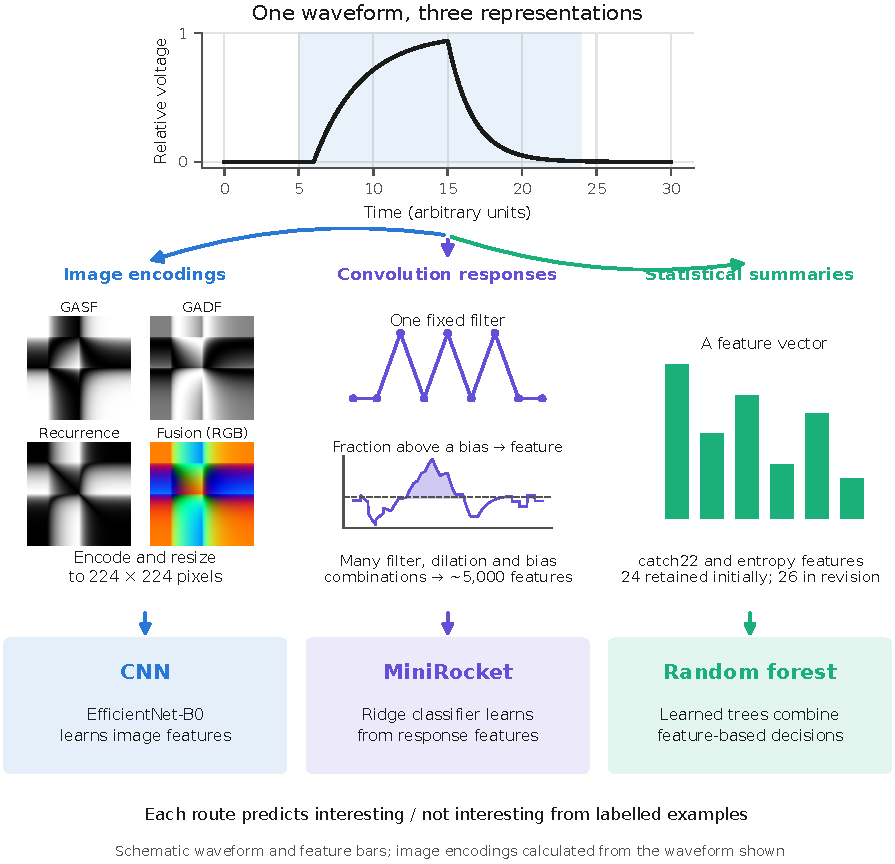
\includegraphics[width=\textwidth]{new/ch8_model_inputs.pdf}
\caption{Three classifier routes from one waveform. The CNN receives image encodings, MiniRocket produces convolution-response features for a ridge classifier, and the random forest receives statistical summaries. GASF, GADF, recurrence and fusion images are calculated from the waveform shown. The waveform, feature bars and single filter response are illustrations, not predictions from a fitted model. The forest experiments retained 24 features initially and 26 in the later revision.}
\label{fig:models}
\end{figure}

\paragraph{Evaluation.}
The models were evaluated through a set of progressively stronger tests. The first forest comparison separated later time blocks from earlier training data, with a gap of at least one window, and reserved four channels for an unseen-channel test. A later blind review queue supplied 1,000 first presentations and 100 repeat presentations. After excluding three unsure and eleven artefact verdicts from the first presentations, 986 windows remained for scoring. This supplied fresh judgements, although some windows overlapped earlier labelled data. Blind review therefore reduced knowledge of the model's prediction without by itself guaranteeing independent training and test signals.

For R4, one recording group was held out at a time. The transform and classifier were fitted using the remaining groups, and only events from the held-out group were evaluated; labelled windows contributed to training only. There were six historical groups drawn from five physical recordings. The separate four-hour MJu26a CH14 excerpt shared signal with the five-channel MJu26a copy, so these two groups were not fully independent. Their dependence is stated with the results.

The original reference CNNs were scored on these same held-out events without retraining. A second CNN comparison then used R4's training examples and recording folds, to separate differences in the training data from differences in model architecture. Finally, the frozen R4 and reference CNN checkpoints were examined against new blind judgements from M4, which had not contributed to R4's training. The sampling plan and model hashes were fixed before these judgements were collected (Appendix~\ref{app:exam}).

\paragraph{Controls and scoring.}
The models were compared with label-shuffle controls and simpler baselines. The initial paired forests were refitted on 200 shuffled training-label sets. The later blind forest analysis instead permuted the evaluation labels 1,000 times against fixed predictions; this tests association between predictions and judgements, rather than the full training procedure. The R4 control used 200 label permutations within recording-group and example-type blocks, refitting the ridge classifier on cached, training-fold MiniRocket features. For computational reasons this null used an unweighted ridge, with the real-label comparison evaluated by the same unweighted procedure. The principal R4 results used class balancing.

Plain accuracy was compared with always predicting the majority class. Balanced accuracy was used to give equal weight to recall of interesting and not-interesting examples. Precision measures how many positive predictions were accepted by the researcher, while recall measures how many human-accepted examples were recovered. Macro F1 averages the F1 score of the two classes. AUC measures ranking: an AUC of 0.97 means that a randomly selected accepted example receives a higher score than a randomly selected rejected example approximately 97\,\% of the time. A high AUC can coexist with weaker classification at a particular threshold. The reported thresholds were a CNN positive-class probability of 0.5 and an R4 ridge decision value of zero, unless stated otherwise.

Confidence intervals used bootstrap resampling appropriate to each experiment: 24-hour channel blocks for the blind window comparisons, resampling within recording groups for the pooled event results, and sampling strata for M4. A second R4 bootstrap resampled whole channel-recording units. Detector agreement and a classifier using only duration, swing and noise measures provided baselines on the same sampled candidate events. All these scores measure agreement with the human reference.

% Sources: docs/rq_roundA/RQ1-cluster-vs-manual-labels.md; saved run79/run1613
% configs and results; W4-A-evaluation.md; rq1b-minirocket-2026-10-20.md;
% rq1b-minirocket-null-2026-10-26.md; rq1b-fair-cnn-2026-10-29.md.
% See data/ch08_verification.json for the saved configuration and exam counts.

\section{Results}

\subsection{Cluster labels against manual labels}

Two random forest models were initially trained on the same signal features, with the difference being how the training windows were labelled. The first classifier used the manual interesting and not-interesting labels. It scored an unseen-channel macro F1 of 0.793, compared with 0.635 for the classifier trained on the four clusters mapped to the same two categories (Table~\ref{tab:forests}). The manual model also scored more highly on a later time block.

\begin{table}[htbp]
\centering
\caption{Initial random forests trained on manual and cluster-derived labels (run 79, M2\_aug, ten-minute windows). Macro F1 with 95\,\% bootstrap intervals; shuffle columns give mean scores after 200 training-label permutations and refits.}
\label{tab:forests}
\small
\begin{tabularx}{\textwidth}{@{}Xrccc@{}}
\toprule
\textbf{Test} & \textbf{$n$} & \textbf{Manual (A)} & \textbf{Cluster (B)} & \textbf{Null A/B}\\
\midrule
Unseen channels & 2,530 & 0.793 [0.764--0.819] & 0.635 [0.594--0.674] & 0.428/0.427\\
Later block & 1,549 & 0.884 [0.798--0.922] & 0.607 [0.524--0.662] & 0.480/0.477\\
\bottomrule
\end{tabularx}
\end{table}

However, the cluster-derived training labels already disagreed substantially with the human reference. Of the 1,271 training windows manually marked interesting, 979 (77\,\%) belonged to clusters mapped to not interesting. The classifier was therefore being taught to reject most of these human-accepted windows before its performance was evaluated. Its lower score reflects this disagreement in the training targets as well as the subsequent classification. It does not establish that clustering is generally unable to organise useful waveform groups.

A later model used seven waveform-shape clusters mapped to interesting or not interesting. Against the blind window labels, it achieved an unseen-channel macro F1 of 0.450 [0.404--0.495], compared with a permutation-null mean of 0.368 ($p=0.001$). Its balanced accuracy was 0.625 [0.586--0.664], with precision 0.256, recall 0.908 and Cohen's $\kappa$ of 0.13. On the later block, macro F1 was 0.482 [0.426--0.536], compared with a null mean of 0.382 ($p=0.001$), with balanced accuracy 0.641 and $\kappa$ of 0.16. The predictions therefore contained information about the human labels, but the high recall came with many rejected windows being flagged.

To compare the practical behaviour of the models, the original manual forest and revised cluster forest were scored on the same 429 blind ten-minute windows (Table~\ref{tab:forestblind}). The manual model was selective: 89\,\% of its positive predictions were accepted, but it found only 41\,\% of the interesting windows. The cluster model recovered 93\,\% of the interesting windows, but only 24\,\% of its positive predictions were accepted. It would therefore present more useful windows for review, alongside a much larger number of rejected ones.

\begin{table}[htbp]
\centering
\caption{Manual forest A and revised seven-cluster forest B2 on the same blind ten-minute windows. The no-earlier-label subset excludes overlap with earlier labelled spans; M2\_concat is a separate recording. These are overlapping subsets, not additional independent tests. Precision and recall refer to the interesting class.}
\label{tab:forestblind}
\small
\begin{tabularx}{\textwidth}{@{}Xlrrrr@{}}
\toprule
\textbf{Population} & \textbf{Model} & \textbf{Macro F1} & \textbf{BA} & \textbf{Precision} & \textbf{Recall}\\
\midrule
All ($n=429$) & Manual A & 0.748 & 0.701 & 0.89 & 0.41\\
 & Cluster B2 & 0.440 & 0.630 & 0.24 & 0.93\\
\addlinespace
No earlier label ($n=328$) & Manual A & 0.702 & 0.659 & 0.82 & 0.33\\
 & Cluster B2 & 0.439 & 0.642 & 0.22 & 0.93\\
\addlinespace
M2\_concat ($n=129$) & Manual A & 0.591 & 0.568 & 0.50 & 0.15\\
 & Cluster B2 & 0.380 & 0.608 & 0.13 & 0.85\\
\bottomrule
\end{tabularx}
\end{table}

Removing windows that overlapped an earlier label reduced the manual model's macro F1 to 0.702, against 0.439 for the cluster model. The 95\,\% interval for the paired difference in macro F1 was 0.164--0.357. Balanced accuracy was much closer, at 0.659 and 0.642, because the two models failed in different directions. On M2\_concat, the manual model's macro F1 fell further to 0.591 and recall to 0.15. Only 13 of the 129 windows in this subset were interesting, limiting the precision of the transfer comparison.

The blind sample did not make every comparison independent of training. The original manual forest reserved CH4\_A2, CH8\_B2, CH12\_C2 and CH16\_D2, while the revised forest reserved CH13--16; three of the latter channels were consequently familiar to the manual forest. The revision also changed the number of trees and features, so this later comparison assesses the two complete pipelines rather than isolating label source alone. Overall, the cluster mapping recovered many interesting windows, but assigning whole shape groups a single binary label did not reproduce the finer distinctions made during human review.

% Sources: RQ1-cluster-vs-manual-labels.md; rq1-v2-blind-2026-10-26.md;
% data/rq1_v2_blind/run79_armA_vs_run1613_10min.json.

\subsection{The CNNs}

The convolutional neural networks were trained on time series data transformed into GASF, GADF, recurrence and fusion images, as described in Chapter~\ref{ch:early}. On an initial 80:20 training and test split, the models scored approximately 91--92\,\% plain accuracy. However, the windows overlapped and were randomly assigned to the two sets, so training and test examples could share signal content. That result established that the models could learn the supplied labels, but gave a limited estimate of performance on independent data.

The later blind window evaluation gave a more conservative assessment (Table~\ref{tab:cnns}). At ten minutes, balanced accuracy was 0.78--0.83 and AUC was 0.93--0.96 across the 429 windows pooled from M2\_aug and M2\_concat. Plain accuracy was still 0.90--0.92, but always predicting not interesting already scored 0.814 because only 80 windows were interesting. Balanced accuracy therefore gives a clearer account of both classes.

\begin{table}[htbp]
\centering
\caption{Reference CNNs against blind window labels (queue 3), at a probability threshold of 0.5. Cells give balanced accuracy, with AUC in parentheses. Pooled rows combine M2\_aug and M2\_concat; they are not wholly independent of the training recording.}
\label{tab:cnns}
\small
\begin{tabularx}{\textwidth}{@{}Xrcccc@{}}
\toprule
\textbf{Windows} & \textbf{$n$} & \textbf{GASF} & \textbf{GADF} & \textbf{Recurrence} & \textbf{Fusion}\\
\midrule
10\,min, pooled & 429 & 0.82 (0.96) & 0.83 (0.95) & 0.79 (0.95) & 0.78 (0.93)\\
10\,min, M2\_concat & 129 & 0.68 (0.90) & 0.63 (0.90) & 0.68 (0.91) & 0.64 (0.81)\\
30\,min, M2\_concat & 114 & 0.86 (0.92) & 0.87 (0.91) & 0.80 (0.91) & 0.77 (0.91)\\
1\,min, pooled & 185 & 0.49 (0.42) & 0.51 (0.46) & 0.39 (0.30) & 0.43 (0.42)\\
\bottomrule
\end{tabularx}
\end{table}

M2\_aug contributed to the earlier training data, so blind judgements on this recording do not establish transfer to an unseen recording. M2\_concat provided the stronger recording-transfer test, although the exact training provenance of the reference checkpoints was incompletely recorded. At ten minutes, its balanced accuracy was 0.63--0.68, with only 13 interesting windows. For example, GASF scored 0.68 [0.54--0.81]. AUC remained 0.81--0.91, indicating that the ranking was more useful than the classifications at the chosen threshold. Lower thresholds improved balanced accuracy on these same labels; this was a threshold inspection, rather than a new independent validation.

The effect of duration was also substantial. On the 30-minute M2\_concat windows, GASF and GADF reached balanced accuracies of 0.86 and 0.87. At one minute, all four models performed poorly, with balanced accuracy of 0.39--0.51 and AUC of 0.30--0.46. On a separate whole-channel scan, they marked approximately 95--96\,\% of one-minute windows interesting. Simply resampling a different duration to the required input length did not make it equivalent to the ten-minute examples used for training. The 30-minute results support some transfer of scale, but do not directly validate the one-hour detector templates, for which no equivalent human-labelled window set was available.

% Source: docs/prompts/blocks/reports/W4-A-evaluation.md.
% Corrected the old table: 0.78--0.83 is the pooled 429-window result, not M2_aug alone.

\subsection{MiniRocket on judged events}

MiniRocket R4 was trained using the larger collection of reviewed candidates, with labelled windows added to its training data. When recording groups were held out in turn, it achieved a pooled AUC of 0.971 [0.965--0.977] and balanced accuracy of 0.919 [0.907--0.930] (Table~\ref{tab:r4}). Each of the five main recording groups had an AUC above 0.95. The results show that the collected labels contained distinctions that could be learned and applied beyond individual examples and channels.

\begin{table}[htbp]
\centering
\caption{MiniRocket R4 with one recording group held out at a time. Intervals are 95\,\% bootstrap intervals. The five main groups are shown separately; the pooled 2,456 events also include 12 events from the overlapping MJu26a CH14 excerpt. The null uses an unweighted ridge, whose real-label pooled balanced accuracy was 0.915 rather than the class-balanced R4 value of 0.919.}
\label{tab:r4}
\small
\begin{tabular}{lrr}
\toprule
\textbf{Held out} & \textbf{AUC} & \textbf{Balanced accuracy}\\
\midrule
CO\_fs2 & 0.989 [0.976--0.998] & 0.954 [0.923--0.981]\\
LM\_fs2 & 0.995 [0.990--0.999] & 0.955 [0.931--0.977]\\
MJu26a (CH10, 13--16) & 0.984 [0.972--0.992] & 0.925 [0.895--0.950]\\
M2\_aug & 0.951 [0.938--0.963] & 0.886 [0.866--0.904]\\
M2\_concat & 0.961 [0.927--0.987] & 0.909 [0.869--0.947]\\
\midrule
Pooled & 0.971 [0.965--0.977] & 0.919 [0.907--0.930]\\
Shuffle null, pooled mean (max) & 0.420 (0.495) & 0.443 (0.492)\\
\bottomrule
\end{tabular}
\end{table}

The label-shuffle control supported this result. None of the 200 permutations reached the real-label score for either AUC or balanced accuracy on the five main recording groups, giving $p=1/201\approx0.005$, the smallest value this number of draws can resolve. The pooled null AUC was 0.420, although each recording's null mean was close to 0.5. Pooling combines scores from different fitted models: their intercepts follow the training class proportions, which can oppose the held-out recording's proportions. This shifts the pooled shuffled ranking below 0.5. The per-recording comparisons provide the clearer interpretation of performance against chance.

On the same 1,689 candidates from the stratified detector-review queues, R4 ranked accepted events with an AUC of approximately 0.97, compared with 0.86 for counting agreeing detectors and 0.90 for the duration, amplitude and noise features alone. Within individual detector families, the event-only variant retained AUC values of 0.88--0.99. Its performance therefore was not explained solely by recognising the proposing detector's typical acceptance rate. These checks support useful distinctions within candidate groups, although they do not isolate waveform shape from every possible correlate of the human judgement. The earlier queue-25-only pilot was superseded by this larger evaluation.

Resampling whole channel-recording units, rather than individual events, gave pooled AUC 0.971 [0.962--0.980] and balanced accuracy 0.919 [0.902--0.935] across 46 such units. This accounts for some dependence within channels, but cannot remove the historical overlap between the MJu26a groups. The 12-event CH14 excerpt is omitted as a separate table row because it shares signal with the five-channel copy. Conversely, when the five-channel group was held out, 12 of its 2,085 training events came from that excerpt. The pooled figures retain those 12 events and should be read with this limitation.

% Sources: rq1b-minirocket-2026-10-20.md; rq1b-minirocket-null-2026-10-26.md.
% The 0.90 scalar baseline is for the 1,689 queue candidates; 0.84 concerns a different event-only comparison.

\subsection{CNN against MiniRocket on the same events}

The original reference CNNs were next shown the same 2,456 events used to evaluate R4 (Table~\ref{tab:cnnvsr4}). Their pooled AUC was 0.722--0.790, compared with R4's 0.971. The strongest reference encoding, GADF, was lower by approximately 0.18, with a paired 95\,\% interval of 0.16--0.20 for R4 minus GADF. However, these CNNs had learned from earlier fixed-window labels, while R4 had learned from reviewed candidate spans with context. This comparison therefore combined a change in model architecture with a change in the examples used to teach it.

\begin{table}[htbp]
\centering
\caption{AUC of the original reference CNNs and MiniRocket R4 on the same 2,456 judged events. R4 uses held-out recording-group predictions; the reference checkpoints are applied without retraining and have incompletely recorded training provenance. The pooled row includes the 12-event MJu26a excerpt, omitted as a separate row.}
\label{tab:cnnvsr4}
\small
\begin{tabularx}{\textwidth}{@{}Xrrrrr@{}}
\toprule
\textbf{Recording} & \textbf{R4} & \textbf{GASF} & \textbf{GADF} & \textbf{Recurrence} & \textbf{Fusion}\\
\midrule
CO\_fs2 & 0.989 & 0.740 & 0.803 & 0.684 & 0.785\\
LM\_fs2 & 0.995 & 0.676 & 0.720 & 0.586 & 0.636\\
MJu26a (CH10, 13--16) & 0.984 & 0.791 & 0.869 & 0.766 & 0.783\\
M2\_concat & 0.961 & 0.573 & 0.608 & 0.568 & 0.585\\
M2\_aug & 0.951 & 0.796 & 0.838 & 0.801 & 0.801\\
\midrule
Pooled & 0.971 & 0.737 & 0.790 & 0.722 & 0.738\\
\bottomrule
\end{tabularx}
\end{table}

A matched-data comparison was therefore performed, training EfficientNet-B0 on R4's examples using the same recording folds. GASF, GADF and fusion encodings were each trained for 12 epochs, using a batch size of 64, learning rate of 0.001 and one fixed random seed. No augmentation or hyperparameter search was performed. The 18 tasks covered three encodings and six folds.

With the training examples and folds aligned, pooled CNN AUC increased to 0.970--0.973, compared with 0.971 for R4 (Table~\ref{tab:faircnn}). Every paired interval included zero, both pooled and by recording. Balanced accuracy was 0.915--0.916, compared with R4's 0.919. These results did not establish an advantage for either architecture on this comparison. The initial gap could not be attributed to CNN architecture alone: training on examples appropriate to the candidate-review task brought the CNNs to a similar level.

\begin{table}[htbp]
\centering
\caption{Matched-data comparison: EfficientNet-B0 trained on R4's rows and recording folds, evaluated on the same 2,456 events. Pooled 95\,\% intervals and paired AUC differences use bootstrap resampling within recordings. The pooled row includes the 12-event overlapping excerpt.}
\label{tab:faircnn}
\small
\begin{tabularx}{\textwidth}{@{}Xrrrr@{}}
\toprule
\textbf{Held out} & \textbf{R4} & \textbf{GASF} & \textbf{GADF} & \textbf{Fusion}\\
\midrule
CO\_fs2 & 0.989 & 0.986 & 0.988 & 0.987\\
LM\_fs2 & 0.995 & 0.997 & 0.998 & 0.998\\
MJu26a (CH10, 13--16) & 0.984 & 0.979 & 0.978 & 0.983\\
M2\_concat & 0.961 & 0.960 & 0.971 & 0.946\\
M2\_aug & 0.951 & 0.957 & 0.951 & 0.960\\
\midrule
Pooled & 0.971 & 0.971 & 0.970 & 0.973\\
95\,\% interval & 0.965--0.977 & 0.965--0.977 & 0.964--0.975 & 0.967--0.978\\
R4 minus CNN & -- & 0.000 & $+0.001$ & $-0.002$\\
Paired 95\,\% interval & -- & $[-0.006,0.006]$ & $[-0.005,0.007]$ & $[-0.007,0.004]$\\
\bottomrule
\end{tabularx}
\end{table}

The shared recording folds also shared the MJu26a overlap described above. In addition, one random seed without tuning cannot establish that these are the best results available from either model family. R4 remained the model selected for the original M4 examination because it could run without a GPU and had already been frozen before the new human labels were collected. The retrained CNNs were not added to that examination, so their comparable performance is demonstrated on the shared recording folds only. The short GPU task times in this experiment do not constitute a hardware-matched comparison of training cost.

% Sources: reference_comparison.json; rq1b-fair-cnn-2026-10-29.md and .json;
% Appendix G, Round 5 (retrained CNNs excluded from the original frozen M4 exam).

\subsection{The held-out exam}
\label{sec:classifierexam}

The original M4 examination tested the frozen R4 and reference CNN models against a newly judged sample of candidates. M4 contained 505 hours across 16 channels. Its pool contained 832,136 candidate events, from which 290 were sampled across detector-agreement and rare-detector strata. The sample was judged with model scores and proposal sources hidden. R4's training excluded M4, although the recording had been used for earlier exploratory runs and a detector sweep; it was not an entirely unseen recording for the researcher. Table~\ref{tab:exposure} records this prior exposure and the subsequent freeze.

Of the 290 judgements, 14 were unsure, leaving 276 answered items for the candidate-acceptance estimates. The frozen classifier scorer mapped interesting to positive, not interesting and artefact to negative, and did not map the seven seed verdicts. This left 269 eligible binary labels. Twelve of those spans could not be read because more than 5\,\% of their samples were missing, leaving 257 cases for the classifier comparison: 59 positive and 198 negative. The five artefacts remain negative examples under this examination rule, despite being excluded from R4's training. These published rules are retained rather than retrospectively changing the labels or rescoring the examination.

On these 257 cases, R4 achieved AUC 0.98 [0.97--0.99] and balanced accuracy 0.93 [0.88--0.97], consistent with its earlier recording-group evaluation (Table~\ref{tab:exam}). At the frozen threshold it produced 52 hits, six false alarms, seven misses and 192 correct rejections. Detector agreement scored AUC 0.85 on the same cases. The reference CNNs reached AUC 0.59--0.66, approximately 0.33--0.40 below R4. This confirms the advantage over those frozen reference models on the new judgements, while leaving the transfer performance of the later retrained CNNs untested.

\begin{table}[htbp]
\centering
\caption{Original M4 classifier examination, scored once on 28 October: 257 readable cases with labels mapped by the frozen scorer. Within-stratum bootstrap 95\,\% intervals. Unweighted performance is the pre-specified primary measure; design weighting represents the candidate pool rather than the sampled mixture. The retrained, matched-data CNNs are not included.}
\label{tab:exam}
\footnotesize
\begin{tabularx}{\textwidth}{@{}>{\raggedright\arraybackslash}Xrrr@{}}
\toprule
\textbf{Model} & \textbf{AUC} & \textbf{Balanced accuracy} & \textbf{AUC minus R4}\\
\midrule
MiniRocket R4 & 0.98 (0.97--0.99) & 0.93 (0.88--0.97) & --\\
\quad design-weighted & 0.96 (0.92--1.00) & 0.77 (0.67--0.92) & \\
GASF CNN & 0.61 (0.55--0.67) & 0.62 (0.56--0.69) & $-0.37$ ($-0.43$ to $-0.31$)\\
GADF CNN & 0.66 (0.60--0.71) & 0.67 (0.61--0.73) & $-0.33$ ($-0.39$ to $-0.27$)\\
Recurrence CNN & 0.64 (0.58--0.70) & 0.68 (0.63--0.74) & $-0.34$ ($-0.41$ to $-0.28$)\\
Fusion CNN & 0.59 (0.53--0.65) & 0.63 (0.57--0.69) & $-0.40$ ($-0.46$ to $-0.33$)\\
Detector agreement & 0.85 & -- & \\
\bottomrule
\end{tabularx}
\end{table}

The sample deliberately gave space to candidates at different agreement levels and from rarely firing detectors. Its unweighted results therefore describe that sampled mixture. After weighting back to the candidate pool, R4's AUC remained high at 0.96 [0.92--1.00], but balanced accuracy fell to 0.77 [0.67--0.92]. Low-agreement candidates made up most of the pool, so the small number of accepted examples in these strata received greater weight. The ranking remained useful, while classification at the chosen threshold was less consistent for the population represented by these weights.

The separate candidate-acceptance analysis, which included all 276 answered judgements and counted seed as accepted, estimated that approximately 10\,\% [6--14\,\%] of M4's candidate pool would be accepted by the researcher. Acceptance increased from 0\,\% at one or two agreeing detectors to 3\,\%, 16\,\%, 35\,\% and 53\,\% across the subsequent agreement bins. Among the detector families, drop v1 had an estimated acceptance of 64\,\% [43--86\,\%] from 14 sampled candidates, followed by BEADS at 45\,\%, wavelet-encoded at 38\,\% and drop v5 at 36\,\%. Matrix-profile acceptance was zero in the sample, while the wavelet prototype was close to zero and symbol search approximately 1\,\%. These are M4-specific estimates with unequal and sometimes small family samples; they supplement the earlier five-recording results in Chapter~\ref{ch:rq1}.

Figures~\ref{fig:m4beforeafter} and \ref{fig:r4examples} show what the scores mean on the signal. The first links candidate scoring to a broad recording view and confirmed events. The second includes false alarms and missed events, so the strong aggregate scores can be considered alongside their practical failures. During judging, M4's unit was declared as volts so that Review could draw its traces. Both scorers already treated an undeclared unit as volts, so this metadata change did not alter the scores (Appendix~\ref{app:exam}).

\begin{figure}[htbp]
\centering
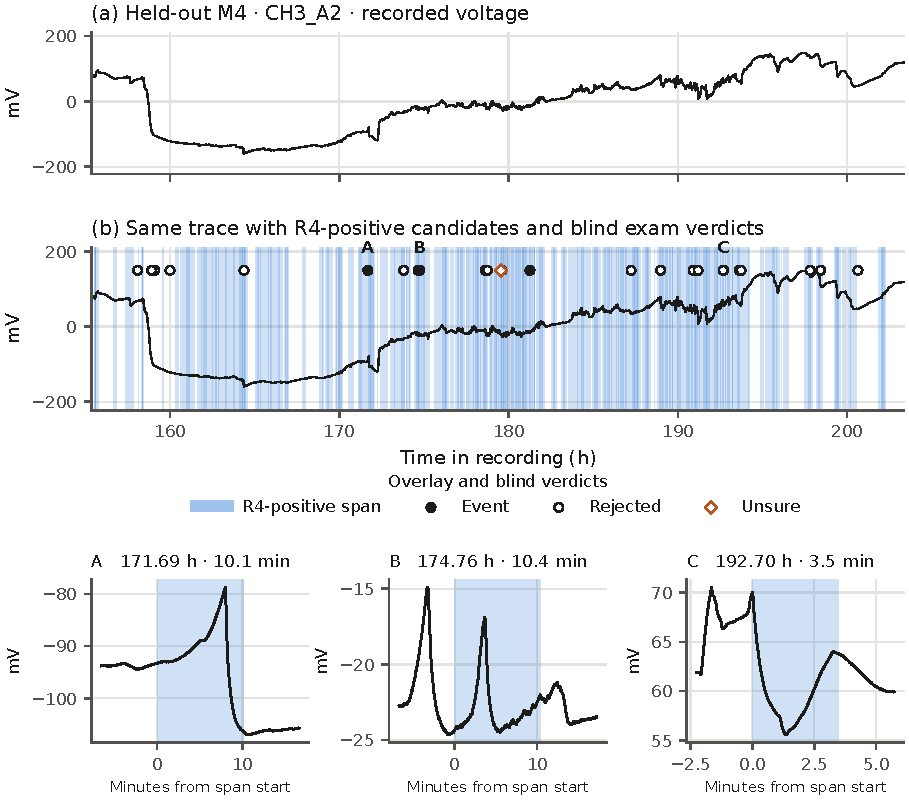
\includegraphics[width=\textwidth]{new/ch8_m4_before_after.pdf}
\caption{The held-out recording before and after candidate scoring. (a) A 48-hour excerpt of M4 channel CH3\_A2. (b) Blue bands show detector-proposed spans of up to 30 minutes that the frozen R4 scores as events, with overlapping proposals suppressed for display. Markers show the blind verdicts on the 25 exam items in this excerpt. R4 agrees on all 24 answered items, and one was judged unsure. A--C zoom in on three confirmed events at their original voltage and time scales, with the judged span shaded. The exam-wide performance is given in Table~\ref{tab:exam}.}
\label{fig:m4beforeafter}
\end{figure}

\begin{figure}[htbp]
\centering
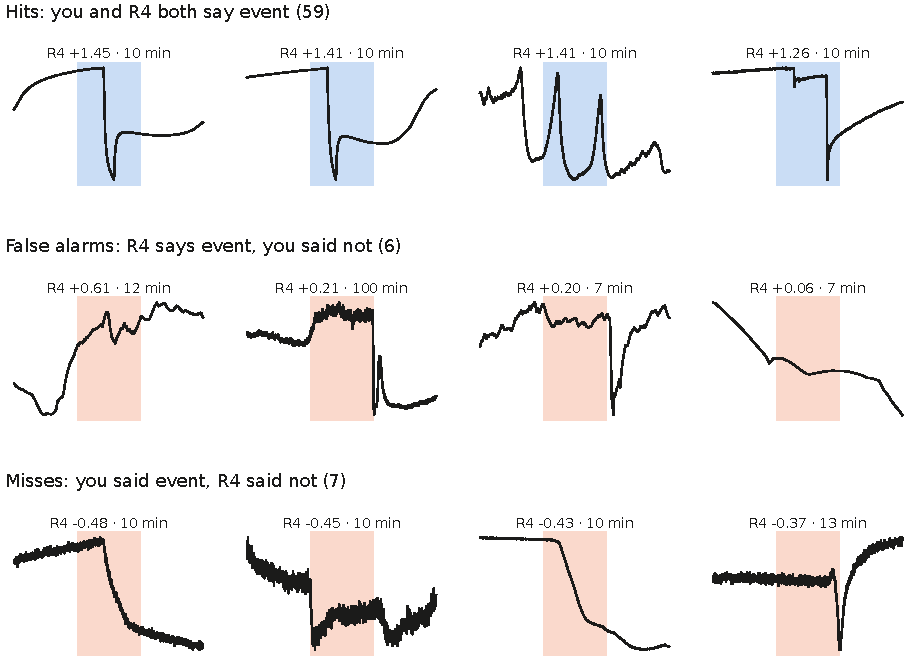
\includegraphics[width=\textwidth]{new/ch8_r4_examples.pdf}
\caption{What R4 gets right and wrong on the original M4 classifier examination, at its pre-specified threshold: among 257 scored cases, 52 hits, six false alarms, seven misses and 192 correct rejections. Shown are the most confident hits, the most confident false alarms and the clearest misses, each judged span shaded with its own length of context on either side. Each panel has its own scale; R4's decision value and the span duration are shown above.}
\label{fig:r4examples}
\end{figure}

% Sources: DATA/derived/exam/M4/results.json and manifest.json; m4_exam_score.Y;
% wave1/data/m4_exam/exam_items.csv; rq1b-fair-cnn-2026-10-29.md.
% 276 answered is the candidate-estimation denominator, not the classifier denominator.
% No model, scorer, threshold or historical result was changed during prose integration.

\section{Discussion}

In response to the research question, the answer was affirmative: data labelled through MycoWave can be used to train classifiers that identify human-accepted events beyond their own training pools. The MiniRocket R4 classifier achieved a pooled AUC of 0.971 and balanced accuracy of 0.919 on held-out recording groups. On the blind-scored M4 examination, it achieved an AUC of 0.98 and balanced accuracy of 0.93. These results suggest that the collected labels contain meaningful patterns that can be learned and applied across datasets. When comparing the same sampled candidates, R4 also ranked human-accepted events more effectively than detector agreement alone, providing a further means of prioritising promising candidates for review.

Comparing the labelling processes revealed that the training labels were an important determining factor in the outcomes. The initial forest comparison used binary manual labels and labels assigned to four automatically generated clusters, which were then mapped to the same interesting and not-interesting categories. Many windows manually marked interesting belonged to clusters assigned a not-interesting label. The resulting classifier was therefore being taught a distinction that already disagreed with the human reference. The later seven-cluster model recovered most of the windows judged interesting, but also flagged many rejected windows. Clustering remained useful for organising similar signal shapes, while assigning whole clusters to interesting or not interesting was too broad to reproduce the researcher's judgements reliably. Similarity between waveforms did not necessarily imply that every member of a cluster should receive the same label.

Comparison of the CNN and MiniRocket classifiers further demonstrated the importance of the training examples. The earlier reference CNNs, trained on manually labelled windows before R4, performed substantially worse on the newer reviewed candidate events. However, when the CNNs were trained on the same examples and recording folds, their pooled AUC increased to 0.970--0.973, with no clear difference from R4 within the uncertainty of the comparison. The initial gap could therefore not be attributed to classifier architecture alone. Providing the CNNs with training examples that matched the evaluation task brought their performance to a similar level. R4 remained a practical choice because it required no GPU and had been frozen before the M4 judgements were collected. The retrained CNNs were not included in that examination, so their comparable performance is established for the shared-fold comparison.

The M4 examination also illustrated why the composition of an evaluation sample matters. The models were fixed first, and the researcher then judged a shuffled queue of 290 candidates without seeing their model scores or proposal sources. After judging, both R4 and the original reference CNNs scored the same eligible spans. Their scores were converted into interesting or not-interesting predictions at the frozen thresholds and compared with the human verdicts. Exclusions under the frozen scoring rules left 257 readable cases for this comparison (Section~\ref{sec:classifierexam}).

R4's balanced accuracy of 0.93 means that its recall of human-interesting cases and its recall of human-rejected cases averaged 93\,\%. This is not simply the percentage of all answers it got right. Its AUC of 0.98 means that an accepted candidate received a higher R4 score than a rejected candidate approximately 98\,\% of the time. The review queue deliberately sampled across agreement levels and rarely firing detectors, giving some uncommon candidates more representation than they had in the full pool. When the same scored cases were weighted to represent their proportions in that pool, balanced accuracy fell to 0.77, while AUC remained high at 0.96. This involved no new model or second set of judgements: each case was given a different weight in the calculation. Low-agreement candidates were much more numerous in the full pool, so errors involving the few accepted examples in these strata had greater influence. R4 therefore retained a strong ability to rank candidates, while its interesting/not-interesting decisions at the chosen threshold were less consistent for the population represented by those weights.

The main limitation remains the human reference itself. The labels were supplied by a single researcher, whose repeated judgements agreed approximately 94\,\% of the time. This demonstrates uncertainty in the reference against which the models were assessed. That agreement percentage is a different measure from balanced accuracy and should not be treated as a strict numerical ceiling. A classifier may learn the researcher's preferences and biases alongside the waveform patterns that informed their decisions. Agreement between multiple reviewers would provide a stronger assessment of whether the learned distinction is shared more broadly.

The reported performance also applies primarily to detector-proposed candidates. R4 was trained to assess spans that had already been selected, with context around them. These results do not establish its performance as a continuous scan of an otherwise unexamined recording, or its ability to recover events that every detector missed. Some historical recording folds also shared signal content through the MJu26a excerpt, limiting the independence of those particular comparisons. The separate M4 examination provides stronger evidence of transfer beyond the development recordings.

The classifiers currently distinguish human-adjudicated interesting events from not-interesting events, rather than identifying specific waveform families. The future scope of this work is to extend the Library sufficiently to develop large, consistently labelled family sets with examples of the variation within each. For example, grouping g-11 assigned 817 de-duplicated events to 42 families, averaging 19.5 events per family. Of these, 519 human-accepted events occupied 41 families, averaging 12.7 accepted events per family. These are Library events, separate from the fixed-window manual labels used in the earlier training experiments (Section~\ref{sec:families}). Several hundred verified examples per family would be a useful collection target, but 500 should not be treated as a universal minimum: the required number depends on the variation and separation of the classes and should be assessed using held-out learning curves. Additional background and unfamiliar examples would also be needed if the classifier were to judge arbitrary windows. The current results support using accumulated human judgements to build a useful candidate-scoring and prioritisation system. Improving the training labels and matching evaluation to intended use are central to continuing to develop that system further.

% Revised 8 Nov 2026 from the author's replacement 8.4. M4 chronology and weighted
% interpretation checked against frozen manifest/results; family counts from
% data/library_events_all_active/events_grouping.json. No universal 500-per-class requirement.

The later follow-up reviews expanded the accepted Library to 2,718 reconciled spans (Chapter~\ref{ch:events}). These labels provide additional material for future training. The classifier results reported here retain their original training and evaluation populations: the new drop-transfer and train reviews were completed afterwards. Likewise, the continuing 2\,Hz CNN sweep applies the existing reference models to new recordings; it supplies detector outputs rather than a new trained classifier or a replacement M4 examination.
